\chapter{Comparative Analysis}
\thispagestyle{chapterstart}

In this chapter, we compare various side-channel resistant implementations of the Dilithium signature scheme, focusing on their feasibility and performance on embedded devices. We analyze how different countermeasures, particularly masking and shuffling techniques, impact security and efficiency. Our aim is to assess these implementations through their experimental results, as represented in the provided figures and tables, and discuss their practicality for real-world deployment.

\section{Assessment of the Attack Surface}

Understanding the attack surface of Dilithium implementations is crucial for identifying potential vulnerabilities to side-channel attacks. Table~\ref{tab:attack_surface} summarizes key findings from studies that evaluated the susceptibility of unprotected Dilithium implementations to such attacks.

\begin{table}[ht]
    \centering
    \renewcommand{\arraystretch}{1.2}
    \caption{Assessment of the Attack Surface in Dilithium Implementations}
    \label{tab:attack_surface}
    \begin{tabularx}{\textwidth}{|X|X|X|}
        \hline
        \textbf{Approach}                                             & \textbf{Evaluation Methodology}                        & \textbf{Findings}                                 \\ \hline
        Profiling attack on bit-unpacking function \cite{Marzougui22} & Machine learning profiling, integer linear programming & Full recovery of $s_1$ from 756,589 signatures    \\ \hline
        Side-channel attack on NTT \cite{Pessl19}                     & Single-trace analysis, factor graph modeling           & Secret key recovery from single power trace       \\ \hline
        Leakage assessment of unprotected version \cite{Migliore19}   & Welch's $t$-tests (500 traces), single-bit DPA         & Significant leakage observed with only 500 traces \\ \hline
    \end{tabularx}
\end{table}

Marzougui et al.~\cite{Marzougui22} performed a profiling side-channel attack on the bit-unpacking function using machine learning techniques and integer linear programming. By analyzing power traces from 756,589 signatures, they successfully recovered the secret key component $s_1$, highlighting the vulnerability of unprotected implementations.

Pessl et al.~\cite{Pessl19} demonstrated a single-trace side-channel attack on the NTT, using factor graph modeling and belief propagation to recover secret keys from a single power trace, exploiting the deterministic patterns in NTT computations.

Similarly, Migliore et al.~\cite{Migliore19} conducted leakage assessments using Welch's $t$-tests and single-bit \ac{DPA} on 500 traces, detecting significant leakage of sensitive information.

These studies demonstrate that unprotected Dilithium implementations are susceptible to side-channel attacks, necessitating effective countermeasures.


\section{Evaluation of Side-Channel Countermeasures}

To mitigate side-channel vulnerabilities, various countermeasures have been proposed and evaluated. Table~\ref{tab:countermeasures} presents a summary of these methods, their evaluation methodologies, and findings regarding their effectiveness.

\begin{table}[ht]
    \centering
    \renewcommand{\arraystretch}{1.2}
    \caption{Evaluation of Side-Channel Countermeasures for Dilithium}
    \label{tab:countermeasures}
    \begin{tabularx}{\textwidth}{|X|X|X|X|}
        \hline
        \textbf{Countermeasure}                 & \textbf{Evaluation Methodology}              & \textbf{Security Framework}                  & \textbf{Findings}                                                     \\ \hline
        High-order masking \cite{Migliore19}    & Welch's t-tests, single-bit DPA              & \(t\)-probed security, gadget-level security & No detectable leakage; 10,000 traces analyzed                         \\ \hline
        Randomized masking \cite{Azouaoui22}    & Sensitivity analysis                         & Improved sensitivity analysis                & Enhanced leakage protection; prevents trace averaging                 \\ \hline
        Improved masking gadgets \cite{Coron23} & Simulation, proofs, C implementation results & \(t\)-probed, \(t\)-NI, \(t\)-SNI security   & Secure gadgets; improved resistance with ShiftMod gadget              \\ \hline
        Shuffling countermeasures \cite{Ravi20} & Practical evaluation on ARM Cortex-M4        & Randomization entropy metrics                & Reduced traceability; effectiveness varies with shuffling granularity \\ \hline
    \end{tabularx}
\end{table}

Migliore et al.~\cite{Migliore19} implemented high-order masking techniques and evaluated their effectiveness using statistical tests on 10,000 traces. Their findings showed no detectable leakage, confirming the robustness of their countermeasures under the \(t\)-probed security model. Azouaoui et al.~\cite{Azouaoui22} introduced randomized masking schemes based on refined sensitivity analysis, leading to improved protection against side-channel attacks by preventing trace averaging. Coron et al.~\cite{Coron23} proposed new masking gadgets, such as the ShiftMod gadget, and validated their security through simulations and formal proofs, demonstrating enhanced resistance under the \(t\)-SNI security model. Ravi et al.~\cite{Ravi20} explored shuffling techniques and evaluated their effectiveness on an ARM Cortex-M4 microcontroller. Their results indicated reduced traceability, with the level of security improvement depending on the shuffling method used.

\section{Key Generation Performance}

The implementation of side-channel countermeasures can impact the performance of the key generation phase in Dilithium. Figure~\ref{fig:keygen_performance} compares the normalized execution times of different implementations, focusing on masking and shuffling techniques.

\begin{figure}[ht]
    \centering
    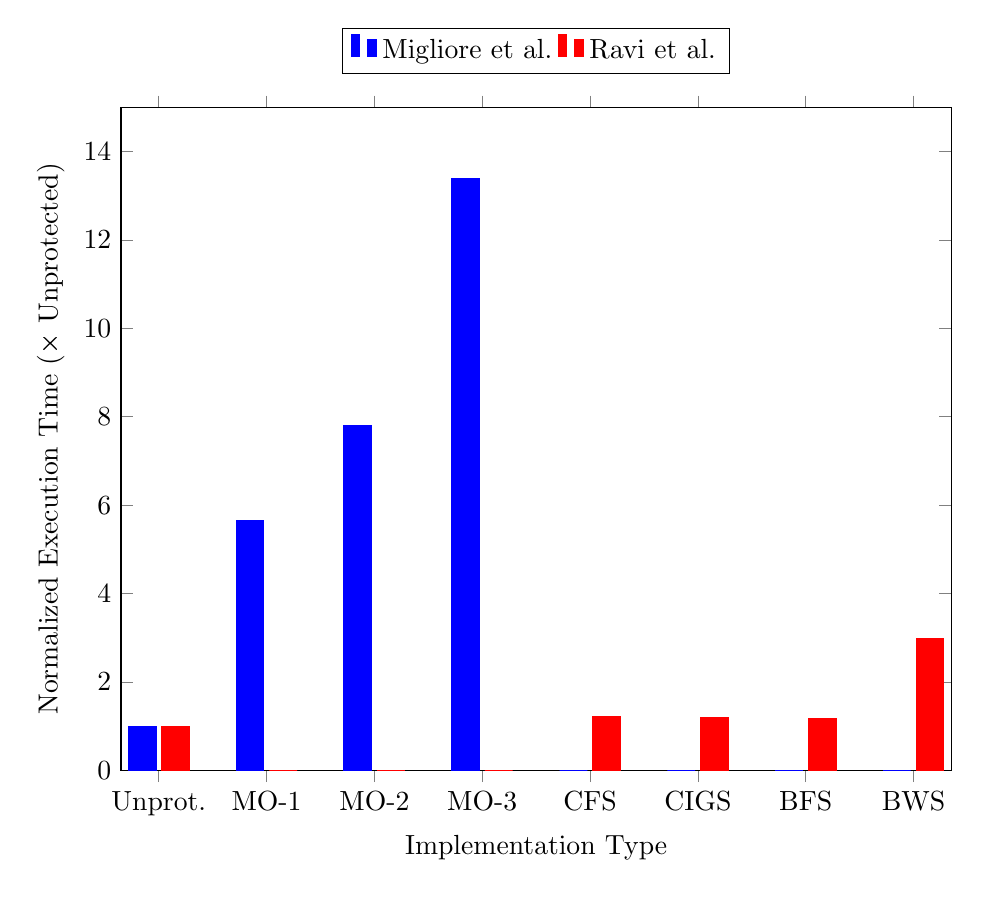
\begin{tikzpicture}
        \begin{axis}[
                ybar,
                bar width=10pt,
                width=\textwidth,
                height=10cm,
                legend style={at={(0.5,1.05)},
                        anchor=south,legend columns=-1},
                symbolic x coords={
                        Unprot.,
                        MO-1,
                        MO-2,
                        MO-3,
                        CFS,
                        CIGS,
                        BFS,
                        BWS
                    },
                xtick=data,
                ylabel={Normalized Execution Time (× Unprotected)},
                xlabel={Implementation Type},
                ymin=0,
                ymax=15,
                enlarge x limits=0.05,
                x tick label style={font=\normalsize},
                y tick label style={/pgf/number format/fixed},
            ]
            \addplot[blue,fill=blue] coordinates {
                    (Unprot.,1)
                    (MO-1,5.66)
                    (MO-2,7.8)
                    (MO-3,13.4)
                    (CFS,0)
                    (CIGS,0)
                    (BFS,0)
                    (BWS,0)
                };

            \addplot[red,fill=red] coordinates {
                    (Unprot.,1)
                    (MO-1,0)
                    (MO-2,0)
                    (MO-3,0)
                    (CFS,1.221)
                    (CIGS,1.203)
                    (BFS,1.181)
                    (BWS,2.971)
                };

            \legend{Migliore et al., Ravi et al.}
        \end{axis}
    \end{tikzpicture}
    \caption{Normalized execution time of Dilithium KeyGen for different implementations.}
    \label{fig:keygen_performance}
\end{figure}

Migliore et al.~\cite{Migliore19} implemented \acp{MO} from 1 to 3. Their results show that higher masking orders significantly increase execution time due to the overhead of processing multiple shares securely. For example, MO-1 incurs approximately 5.66 times the execution time of the unprotected version, while MO-3 increases this to 13.4 times.

Ravi et al.~\cite{Ravi20} evaluated shuffling techniques, including \ac{CFS}, \ac{CIGS}, \ac{BFS}, and \ac{BWS}. Their implementations exhibit a moderate performance overhead, with execution times ranging from 1.18 to 1.22 times the unprotected version for \ac{CFS}, \ac{CIGS}, and \ac{BFS}. The \ac{BWS} implementation has a higher overhead of approximately 2.97 times, due to the increased computational complexity of bitwise shuffling.

The data was collected through benchmarking on ARM Cortex-M4 microcontrollers, representing common embedded platforms. Execution times were measured under controlled conditions to ensure reliable comparisons.

\section{Signing Performance}

The signing operation is another critical aspect affected by side-channel countermeasures. Figure~\ref{fig:combined_performance_updated} illustrates the normalized execution times for various implementations, focusing on masking and shuffling techniques.

\begin{figure}[ht]
    \centering
    \begin{subfigure}[b]{0.45\textwidth}
        \centering
        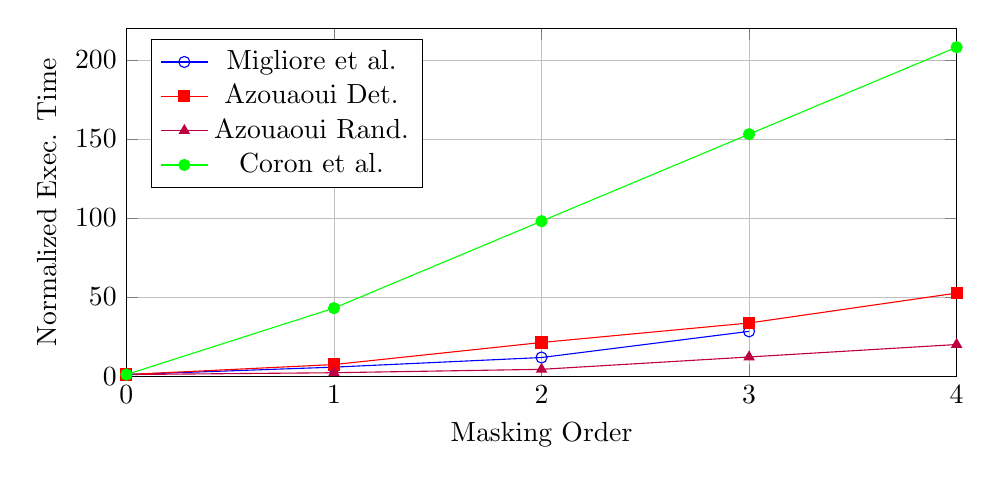
\begin{tikzpicture}
            \begin{axis}[
                    width=\textwidth,
                    height=6cm,
                    xlabel={Masking Order},
                    ylabel={Normalized Exec. Time},
                    xmin=0, xmax=4,
                    ymin=0, ymax=220,
                    xtick={0,1,2,3,4},
                    ytick={0,50,100,150,200},
                    legend pos=north west,
                    grid=both,
                    grid style={line width=.1pt, draw=gray!10},
                    major grid style={line width=.2pt,draw=gray!50},
                ]
                % Migliore data
                \addplot[color=blue,mark=o] coordinates {
                        (0,1)
                        (1,5.68)
                        (2,11.77)
                        (3,28.3)
                    };
                \addlegendentry{Migliore et al.}

                % Azouaoui Deterministic data
                \addplot[color=red,mark=square*] coordinates {
                        (0,1)
                        (1,7.32)
                        (2,21.27)
                        (3,33.6)
                        (4,52.5)
                    };
                \addlegendentry{Azouaoui Det.}

                % Azouaoui Randomized data
                \addplot[color=purple,mark=triangle*] coordinates {
                        (0,1)
                        (1,2.15)
                        (2,4.3)
                        (3,12.11)
                        (4,20)
                    };
                \addlegendentry{Azouaoui Rand.}

                % Coron data
                \addplot[color=green,mark=*] coordinates {
                        (0,1)
                        (1,43)
                        (2,98)
                        (3,153)
                        (4,208)
                    };
                \addlegendentry{Coron et al.}

            \end{axis}
        \end{tikzpicture}
        \caption{Masking Implementations}
        \label{fig:masking_performance_line}
    \end{subfigure}
    \hfill
    \begin{subfigure}[b]{0.45\textwidth}
        \centering
        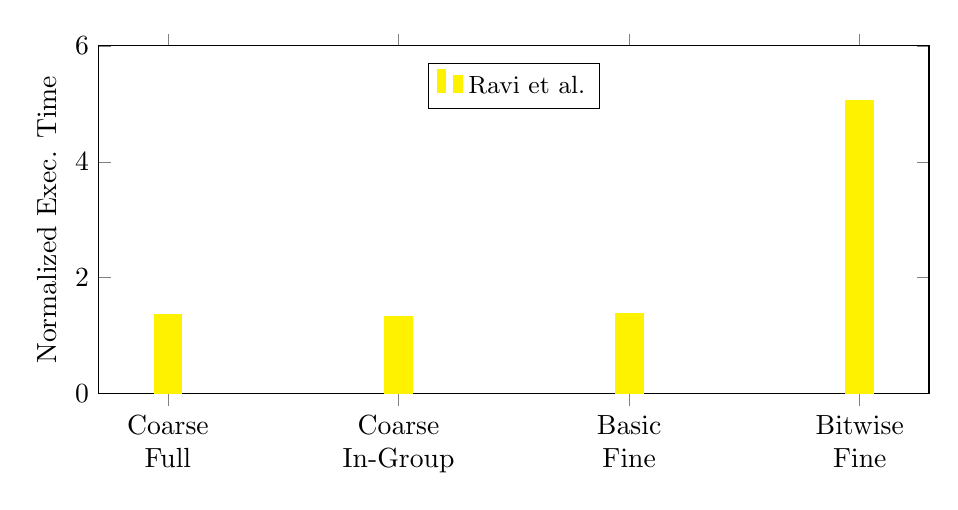
\begin{tikzpicture}
            \begin{axis}[
                    ybar=0pt,
                    bar width=10pt,
                    width=\textwidth,
                    height=6cm,
                    legend style={
                            at={(0.5,0.95)},
                            anchor=north,
                            draw=black,
                            font=\small
                        },
                    symbolic x coords={
                            {Coarse\\Full},
                            {Coarse\\In-Group},
                            {Basic\\Fine},
                            {Bitwise\\Fine}
                        },
                    xtick=data,
                    ylabel={Normalized Exec. Time},
                    ymin=0,
                    ymax=6,
                    enlarge x limits=0.10,
                    x tick label style={font=\normalsize, align=center},
                    y tick label style={/pgf/number format/fixed},
                ]
                \addplot[yellow,fill=yellow] coordinates {
                        ({Coarse\\Full},1.359)
                        ({Coarse\\In-Group},1.338)
                        ({Basic\\Fine},1.377)
                        ({Bitwise\\Fine},5.06)
                    };

                \legend{Ravi et al.}
            \end{axis}
        \end{tikzpicture}
        \caption{Shuffling Implementations}
        \label{fig:shuffle_performance}
    \end{subfigure}
    \caption{Normalized execution time of Dilithium Signing for masking and shuffling implementations.}
    \label{fig:combined_performance_updated}
\end{figure}

In Figure~\ref{fig:masking_performance_line}, the execution times of masking implementations are plotted against the masking order. Migliore et al.~\cite{Migliore19} observed that higher masking orders significantly increase execution time, with MO-1 at approximately 5.68 times the unprotected version and MO-3 reaching 28.3 times. Azouaoui et al.~\cite{Azouaoui22} showed that their randomized masking scheme achieves better performance, with MO-2 at 4.3 times the unprotected execution time, due to more efficient handling of randomness and optimized masking gadgets. Coron et al.~\cite{Coron23} reported even higher overheads, particularly at higher masking orders, reflecting the complexity of their high-order masking gadgets.

Figure~\ref{fig:shuffle_performance} shows the performance impact of shuffling techniques from Ravi et al.~\cite{Ravi20}. The Coarse-Full, Coarse In-Group, and Basic Fine shuffles exhibit moderate overheads (approximately 1.34 times the unprotected version), while the Bitwise Fine shuffle incurs a higher overhead of about 5.06 times, due to the finer granularity of shuffling and increased computational demands.

The execution times were obtained through practical implementations on relevant hardware platforms, such as embedded devices and laptops, ensuring that the performance measurements accurately reflect real-world scenarios and provide a reliable basis for comparative analysis.

\section{Discussion}

The comparative analysis demonstrates that implementing side-channel countermeasures in Dilithium involves trade-offs between security and performance. High-order masking provides strong security guarantees but at the cost of significant execution time increases, which may not be practical for resource-constrained embedded devices. Randomized masking schemes offer a better balance, improving security while mitigating some performance penalties.

Shuffling techniques introduce randomness in operation sequences, reducing the predictability exploited in side-channel attacks. They generally incur lower performance overheads compared to high-order masking but may offer less robust security, depending on the attack model and the granularity of shuffling.

Practitioners must consider the specific security requirements and performance constraints of their applications when choosing countermeasures. For high-security environments where leakage resilience is critical, higher-order masking may be justified despite the overhead. In contrast, applications with stringent performance needs may prefer shuffling or lower-order masking combined with other lightweight countermeasures.

Regular assessment of implementations against emerging side-channel attacks is essential to maintain security. The evolution of attack techniques necessitates continuous evaluation and adaptation of countermeasures to ensure that Dilithium implementations remain both secure and efficient on embedded platforms.
